\begin{surferPage}[216 Tekillik]{Birçok Gerçel Tekillikli Yüzeyler}
Daha önce değindiğimiz gibi, derecesi $7$ olan bir yüzeyin sahip olabileceği en fazla tekillik sayısı (yani $\mu(7)$) bilinmiyor. Bir üst ve alt sınıra sahibiz yalnızca:  $99\le \mu(7) \le 104$. 

Dolayısıyla genel bir $d$ derecesi için daha da az bilinmesi çok şaşırtıcı olmamalı.
Hiç değilse,  Sonja Breske, Oliver Labs ve Duco van~Straten, S.V.\ Chmutov'un bir inşasından yola çıkarak, halihazırdaki en fazla tekillik sayılarının, gerçel tekilliği olan yüzeyler tarafından da gerçeklendiğini gösterebildiler. Şu ana kadar 
    \[0,41\bar{6}d^3 \lessapprox \mu(d) \lessapprox 0.44\bar{4} d^3\]
olduğunu biliyoruz. Aşağıda inşanın simetrisi ve düzlemde bir doğru yerleştirmesinde olabilecek en fazla siyah bölge ile ilişkisi görülebilir.
    \begin{center}
      \begin{tabular}{c@{\qquad}c}
        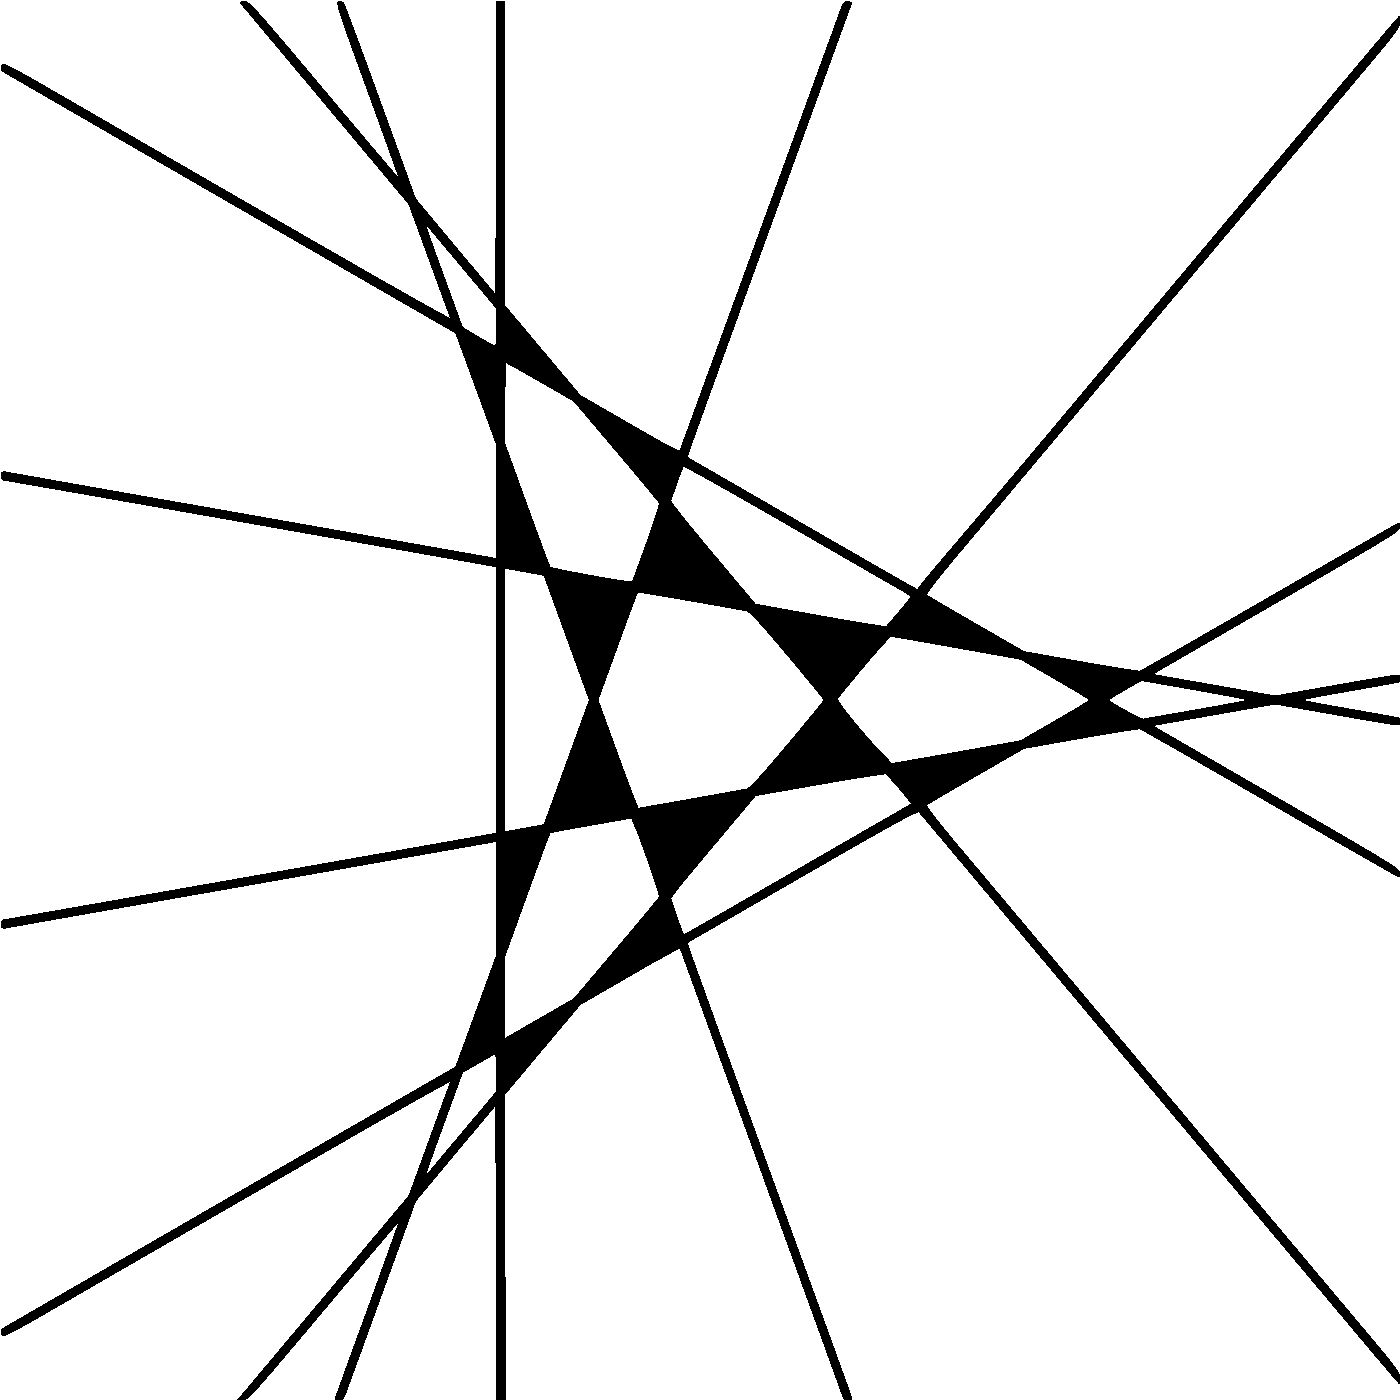
\includegraphics[height=1.5cm]{./../../common/images/vielesing.pdf}
        &
        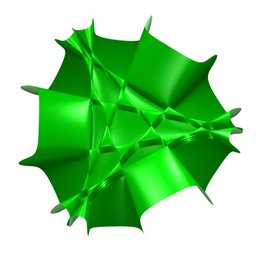
\includegraphics[height=1.5cm]{./../../common/images/p9surface_von_oben}
      \end{tabular}
    \end{center}
\end{surferPage}
